Our initial approach to this problem was to test a variety of distinct classifiers in an effort to improve upon the amount of properly classified elements and determine what classifier would be best to proceed with.

\begin{figure}[h!]
  	\label{compall}
  	\centering
    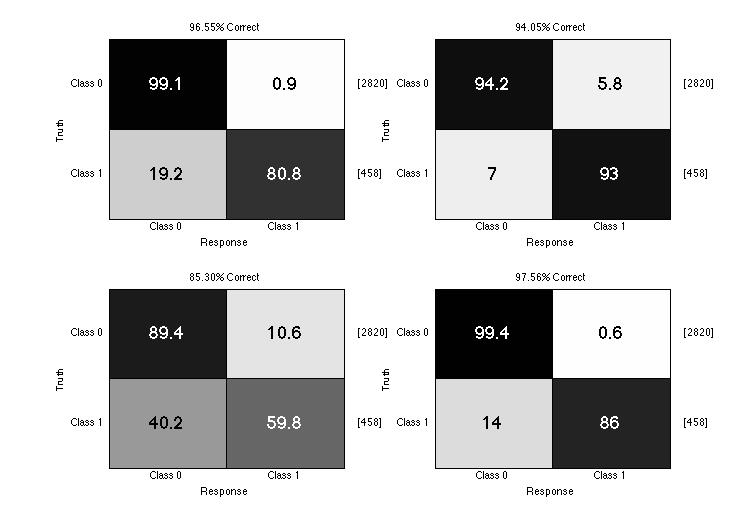
\includegraphics[width=0.5\textwidth]{Figures/allcomp.jpg}
	\caption{Confusion Matrices for KNN (top left), SVM (top right), RVM (bottom left) and Tree Bagger (bottom right)}
\end{figure}

We attempted to classify this data using a Support Vector Machine (SVM), Relevance Vector Machine (RVM), K-Nearest Neighbours, and a Tree Bagger. When choosing these algorithms, it is important to remember that a long training phase is acceptable, as long as the desired algorithm has a quick classification time. The performance of these classifiers was determined using k-folds on our training data with 10 folds. The results of this test are shown in Figures 2.

The results in Figure 1 are displayed as confusion matrices describing the correct classification and misclassification of each classifier. As can be seen the TreeBagger performs the best with about 98\% correct classification in 10 folds. This value is more or less consistent with the results achieved in \cite{adeater}. We were not able to exceed the results of \cite{adeater}. 

The RVM was clearly the worst performing of the algorithms and so we immediately eliminated that as a choice for classifier. It seemed that misclassification of legitimate content was worse than misclassification of advertisements, so we valued very highly the percent of non-ads classified. As such, because of its performance the Tree Bagger became the clear choice for continued work. 

It is also worth noting that there is an inherent bias within the data. There are approximately 2500 examples of advertisements and 500 examples of non-advertisements. We chose to work with all examples for training so that we could make comparisons \cite{adeater}. However, it is possible that this may skew the results slightly.